\documentclass{article}

\usepackage[utf8]{inputenc}
\usepackage[portuges]{babel}
\usepackage{minted}
\usepackage{verbatim}
\usepackage{hyperref}
\usepackage{graphicx}
\usepackage{minted}
\usepackage{color}
\usepackage{subcaption}
\usepackage[dvipsnames]{xcolor}
\usepackage{float}
\usepackage{textcomp}
\usepackage{mathtools}
\usepackage{listings}
\usepackage{tabularx}
\usepackage{xcolor}
\usepackage{amsmath}

\lstset { %
  language=C,
  basicstyle=\footnotesize,% basic font setting
}
\usepackage{textcomp}
\usepackage[a4paper,margin=1in,footskip=0.25in]{geometry}
\newcommand\crule[3][black]{\textcolor{#1}{\rule{#2}{#3}}}


\begin{document}
\begin{titlepage}

  \newcommand{\HRule}{\rule{\linewidth}{0.5mm}} % Defines a new command for the horizontal lines, change thickness here

  \center % Center everything on the page

  \textsc{\large Universidade do Minho}\\[0.5cm] % Name of your university/college
  \textsc{\large Departamento de Informática}\\[2cm] % Major heading such as course name

  \HRule \\[0.4cm]
  { \huge \bfseries Algoritmos Paralelos}\\[0.4cm] % Title of your document
  \HRule \\[1cm]

  { \Huge \bfseries Escalabilidade de diferentes}\\[0.4cm]
  { \Huge \bfseries algoritmos paralelos}\\[3cm] % Title of your document
  
\includegraphics[width=6cm]{logo.png}
  \\[4cm]

  \Large
  António Sérgio Alves Costa \textsc{A78296}\\
  José Pedro Moreira Resende \textsc{A77486}\\[2cm]

  \large 1 de Junho de 2019

\end{titlepage}

\tableofcontents

\newpage

\section{Introdução} 
\par Algoritmos de ordenação sao usados para reorganizar e ordenar uma dada lista ou array de acordo com parametros fornecidos por um comparador de elementos.
\par Existem varios algoritmos de ordenação com diferentes perfis de execucação e memoria, neste artigos vamos falar em especifico do heapsort ,da sua paralelização e da sua caracterização.
\par O heapsort é um algoritmo de ordenação da familia dos algoritmos de ordenacao por seleção. 
\par Este algoritmo usa uma estrutura de dados heap para os ordenar a medida que os insere de forma a tornar a ordenacao estavel. 
\par O seu tempo de execução sobre conjuntos ordenados aleatoriamente é muito bom, tem um uso de memória bem comportado e o seu desempenho em pior caso é praticamente igual ao desempenho em caso médio.

\section{Algortimo: Heapsort} 

\subsection{Sequencial}
Nesta implementação do algoritmo heap sort sequencial utilizamos o codigo disponibilizado no enunciado. 
\par  O funcionamento deste algoritmo consiste em duas fases. Primeiramente e construido uma heap apartir do array  que nos e dado, em segundo é construido o array ordenado retirando o maior numero (root atual) e inserindo no array ordenado. A heap e entao atualizada de forma a manter os invariantes deste tipo de estrutura e eleger um novo root.

\begin{figure}[!htb]
  \centering
  \begin{subfigure}{.5\textwidth}
    \centering
    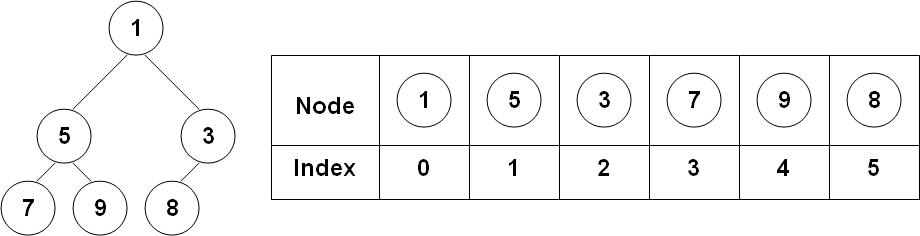
\includegraphics[width=.8\linewidth]{Binary_Heap_with_Array_Implementation.JPG}
  \end{subfigure}%
  \begin{subfigure}{.5\textwidth}
    \centering
    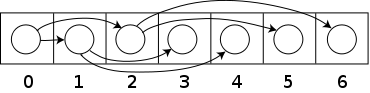
\includegraphics[width=.8\linewidth]{370px-Binary_tree_in_array.png}
  \end{subfigure}
\end{figure}

\par Este array ordenado e na verdade feito no mesmo array da heap e simplesmente e alterado os limites final da heap, reaproveitando a memoria, sem ser necessario alocar um novo array para guardar o resultado final.


\subsection{Paralelo}
Com o intuito de paralelizar e acelarar este algoritmo depois de alguma pesquisa e experimentação chegamos a uma implementação na qual dividimos o array em varias hheaps mais pequenas de tamanho constante (sempre que possivel). 
\par Assim tanto as heaps como os arrays ordenados associados a cada uma destas estruturas podem ser calculados e ordenados de forma independente e paralela. 
\par Utilizamos aqui o scheduler dinamico do omp de forma a distribuir melhor a carga de trabalho entre as threads. 
\par Apos obtermos varios segmentos ordenados e necessario correu o processo de fundir estes segmenetos de forma a obter um unico array ordenado. 
\par Para este trabalho foi usado uma heuristica de redução em arvore o que torna todo o processo de merge extremamente efeciente e possivel de executar de forma paralela, uma vez que temos blocos sem dependencias entre si, tirando partido tambem de um scheduler dinamico de forma a que a carga de trabalho seja distribuida pelas threads.

\section{Apresentação e Análise dos Resultados}
\subsection{Apresentação dos Resultados}
\subsection{Tempos de execuçao}
\begin{figure}[!htb]
  \centering
  \begin{subfigure}{.5\textwidth}
    \centering
    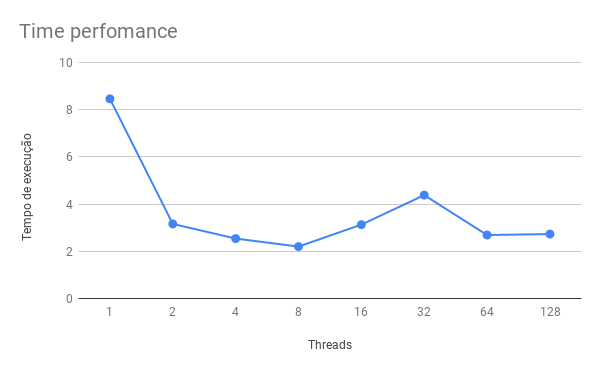
\includegraphics[width=.9\linewidth]{TimePerfomance.png}

  \end{subfigure}%
  \begin{subfigure}{.5\textwidth}
    \centering
    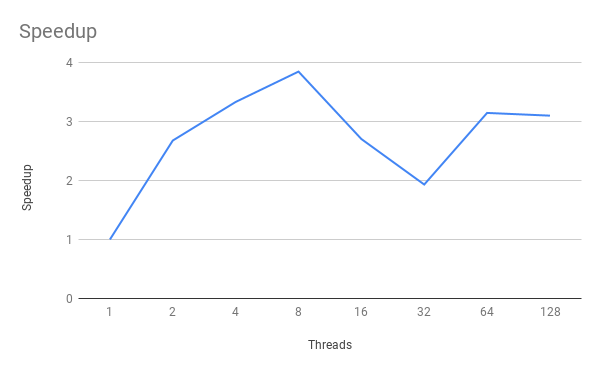
\includegraphics[width=.9\linewidth]{Speedup.png}
  \end{subfigure}
\end{figure}

\subsubsection{Sequencial}

\subsubsection{Paralelo}

\subsection{Análise dos Resultados}

\section{Conclusão}

\clearpage

\end{document}
